\documentclass[../main.tex]{subfiles}

\begin{document}
\chapter{Methodology}
\label{cha:Methodology}
In this chapter I describe in detail the steps outlined in \cref{intro:aims}. In \cref{method:implementation} I discuss the method used and decisions made to create the environment and agents required. In \cref{method:experiments} I discuss the experiments designed to test the hypotheses outlined in \cref{intro:reserach-qs}. 

\section{Implementation} \label{method:implementation}
In order to simplify the process of training RL agents a few changes have been made to the rules mentioned in \cref{intro:rules}. First, jokers are removed -- keeping them in increases the combinatorial complexity of the game, massively increasing the number of actions an RL agent has to learn which is difficult to deal with using my limited compute resources. 

Second, we're only concerned with rounds, rather than the overall game. The meat of playing Yaniv comes from the rounds. There's a bit of meta-game you can play, most of it comes down to strategies to hit exactly 100, but again this would increase the state needed to represent the game and add complexity without much benefit to our research.

\subsection{Simulation Environment}
Any game is interacted with through a series of actions and observations. A player will make an observation, then take an action that results in a new observation. This cycle is implemented for Yaniv in the |yaniv_rl/game| module in a series of Python classes. 

As with most games, Yaniv only allows certain actions to be taken at any point. For instance, you cannot discard a card that you do not hold in your hand. This narrows down the list of possible actions you can take for a given state to the \textit{legal actions}.

Yaniv has two phases per turn, first, the discard phase, the player can discard a legal combination of cards or call Yaniv if their total hand score is less than 8. In the second phase, the draw phase, they can either pick up from the discard pile or draw a card from the deck. A human will usually consider the two phases together and make one action, draw and discard. 

The order of the cards you discard are important in Yaniv, as it dictates what the next player can pick up -- they can pick up either the top or the bottom card. With this in mind, there are 1072 possible legal card combinations that can be discarded. Some of these actions are redundant, however. For example, when discarding a pair the order of the pair is irrelevant since the next player can always pick up either card. When discarding three or four of a kind, which cards are in the middle is important, as they will not be available to the next player. This can be used to deny cards you know the player is trying to collect, by hiding them in the middle of a discard. 

Using this information it is possible to reduce the total number of discard combinations to 484 by ignoring actions with duplicate effects on the game. The algorithm to generate the actions is located in |yaniv_rl/game/jsondata/gen_discard_actions.py|. Discard actions are represented as a string containing the cards to be discarded. A card is encoded as a 2 character string |SUIT + RANK|, where suit is one of |["C", "D", "H", "S"]| and rank is |["A", "2", "3", "4", "5", "6", "7", "8", "9", "T", "J", "Q", "K"]|. So the ace of spades would be |"SA"| and the 5 of Hearts |"H5"|. The possible ways of discarding a three of a kind are: |["D2C2H2", "C2D2H2", "C2H2D2"]|. 

In total there are 488 possible actions a player can take, the 484 discard actions, a |yaniv| action, and 3 pick up actions; |pickup_top_card|, |pickup_bottom_card|, and |draw_card|. When the previous player has only 
discarded single card the two pickup actions are synonymous. 


\subsection{Heuristic Agents} \label{method:rule_agents}
One of the important questions in \cref{intro:reserach-qs} is how skill effects luck, and how different events change with more or less able players. In order to fully test the differences in skill it's important to be able to simulate different levels of ability. One way to do that is to craft heuristic agents based on human knowledge. 

To do this I have created three simple agents. The first is a random action agent which takes random legal actions. This simulates a player with no skill, they only know the rules of the game (i.e. what actions they're allowed to take) but cannot use strategy.

Next is the novice agent, which aims to simulate a new player who has just learned the rules and the basic objective. Often when a new player picks up the game they just put down the highest scoring card in their hand and don't think about making card combinations. While it's possible to win like this, its inefficient.

Finally, the intermediate agent, which implements the basic strategy in Yaniv, which is to build combinations of cards -- even if that means your hand score will temporarily increase. This simulates a player with a few games of experience, they understand the importance of building multiple card combinations but lack further strategy. 

Another important reason for the heuristic agents is to benchmark the RL agent as it trains. Yaniv is a relatively new game with a small player base and so there are no available baselines to test our reinforcement learning agents' performance against.

The strategies for the three agents are outlined below:
\begin{enumerate}
    \item \textbf{Random Action}: Uniformly samples legal actions.
    \item \textbf{Novice Strategy}: Always call Yaniv if the action is available. Discard the highest scoring combination of cards. If the available discard is less than 2, pick it up otherwise draw from the deck. 
    \item \textbf{Intermediate Strategy}: Checks to see if picking up from the discard pile will increase the number of cards that can be discarded next turn. If so pick the highest scoring discard combination that doesn't include the cards used for next turns combinations. Otherwise, act like the novice strategy. 
    \begin{itemize}
        \item This strategy aims to reduce the number of cards in its hand as quickly as possible, usually by making pairs. 
    \end{itemize}
\end{enumerate}

\cref{tab:rules-winrates} details the win rates of each agent. When playing itself the random action agent will often end in a draw. 

\begin{table}[]
\centering
\begin{tabular}{@{}llll@{}}
             & Random & Novice & Intermediate \\
Random       & 0.0674 & 0.0151 & 0.0111       \\
Novice       & 0.9417 & 0.4797 & 0.3231       \\
Intermediate & 0.9842 & 0.6746 & 0.4953      
\end{tabular}
\caption{Rule-based agents' win rates. Represents a tournament Row vs. Column with 10000 games played. A win rate of 0.5 means that the agent on the row won 5000 games against the column agent.}
\label{tab:rules-winrates}
\end{table}

\subsection{Gym Environment}
In order to train an RL agent, the gym environment needs to encode the state into a vector of inputs. The gym environment provides a wrapper around the human-friendly game environment. This project uses Ray's RLlib framework and algorithm implementations \cite{liang_rllib_2018}. RLlib provides a base interface |MultiAgentEnv|, an extension of OpenAI's gym environment for use in a multi-agent setting \cite{brockman_openai_2016,seita_scaling_nodate}. 

\subsubsection{Observation Encoding}
One of the more important steps when designing an RL environment is to come up with an efficient and sensible way to encode the current state into a set of input features for a neural network. The actual learning performance of an RL algorithm can be limited by the design \cite{sutton_reinforcement_2018}. The full state of the game would include the current player's hand and all the actions taken before the current time step. As there is technically no limit to how long a game of Yaniv can last, encoding all this information would lead to a non-stationary and potentially huge state space. Both of these problems can be mitigated by designing a state encoding using human game knowledge. 

\cref{tab:state-enc} shows the initial state encoding chosen for this project. There are 4 main features. They aim to approximate human knowledge at any given step in time. A player knows what is in their hand, what cards have been played and are out of the game, the two possible cards that can be picked up, and how many cards each opponent has left in their hand. A human with perfect memory should also know what cards any opponent has picked up from the discard pile. This is encoded in the known cards feature for each opponent. This can be vital information as it should help avoid making wrong calls. 

\begin{table}[]
\resizebox{\textwidth}{!}{%
\begin{tabular}{@{}lll@{}}
\toprule
Feature             & Size       & Description                                                        \\ \midrule
Current Hand        & 52         & Players current hand                                               \\
Dead cards          & 52         & Discarded cards which are no longer in play                        \\
Top Card            & 17         & \multirow{2}{*}{Available cards to pick up from the previous play} \\
Bottom Card         & 17         &                                                                    \\
Known Cards         & (n-1) * 52 & Known cards in the opponent hands                                  \\
Opponent Hand Sizes & (n-1) * 6  & One-hot encoding of opponent hand size                             \\ 
                    & 58n + 80   &                                                \\ \bottomrule                       
\end{tabular}%
}
\caption{The Yaniv State Encoding.}
\label{tab:state-enc}
\end{table}

In two-player the state vector is of length 196 and in three-player it is 254. It is also possible for an agent trained in three-player to play in two-player games as the inputs for the second opponent are ignored and set to zero. Likewise for a two-player trained agent. 

The current hand, dead cards and known cards are encoded in a vector of length 52, where all inputs are zero unless the card ID is present in the feature. The discards are encoded in a two-plane vector, one for the rank and one for the suit and then concatenated. This state representation was chosen as it includes most of the information that goes into making a decision in Yaniv in a compact way. 

\subsubsection{Action Representation}
% \note{from James: add figs to help show action repr}

As Yaniv is a multi-phase game it is important to decide how the agent will interact with the model. It can either do its two actions sequentially, i.e. calling step with the discard action, then receiving a new observation and calling step again with the pickup action. Or it can take two actions at once, telling the environment to step with both its discard and pick up action. 

The output of the policy network is the same length as the number of actions. It's normalised by a |softmax| function, so the output is a list of probabilities each one corresponding to a distinct action. 

To implement the second action representation you have to create a separate action for each combination of discard and pickup, i.e. the cross product of the discard action and the pickup actions. The Yaniv action is still a separate action. This means that the total number of actions is now almost tripled to \numprint{1462}. This causes the algorithm to train far slower as shown in \cref{fig:multi_vs_single_actions}.

\begin{figure}
    \centering
    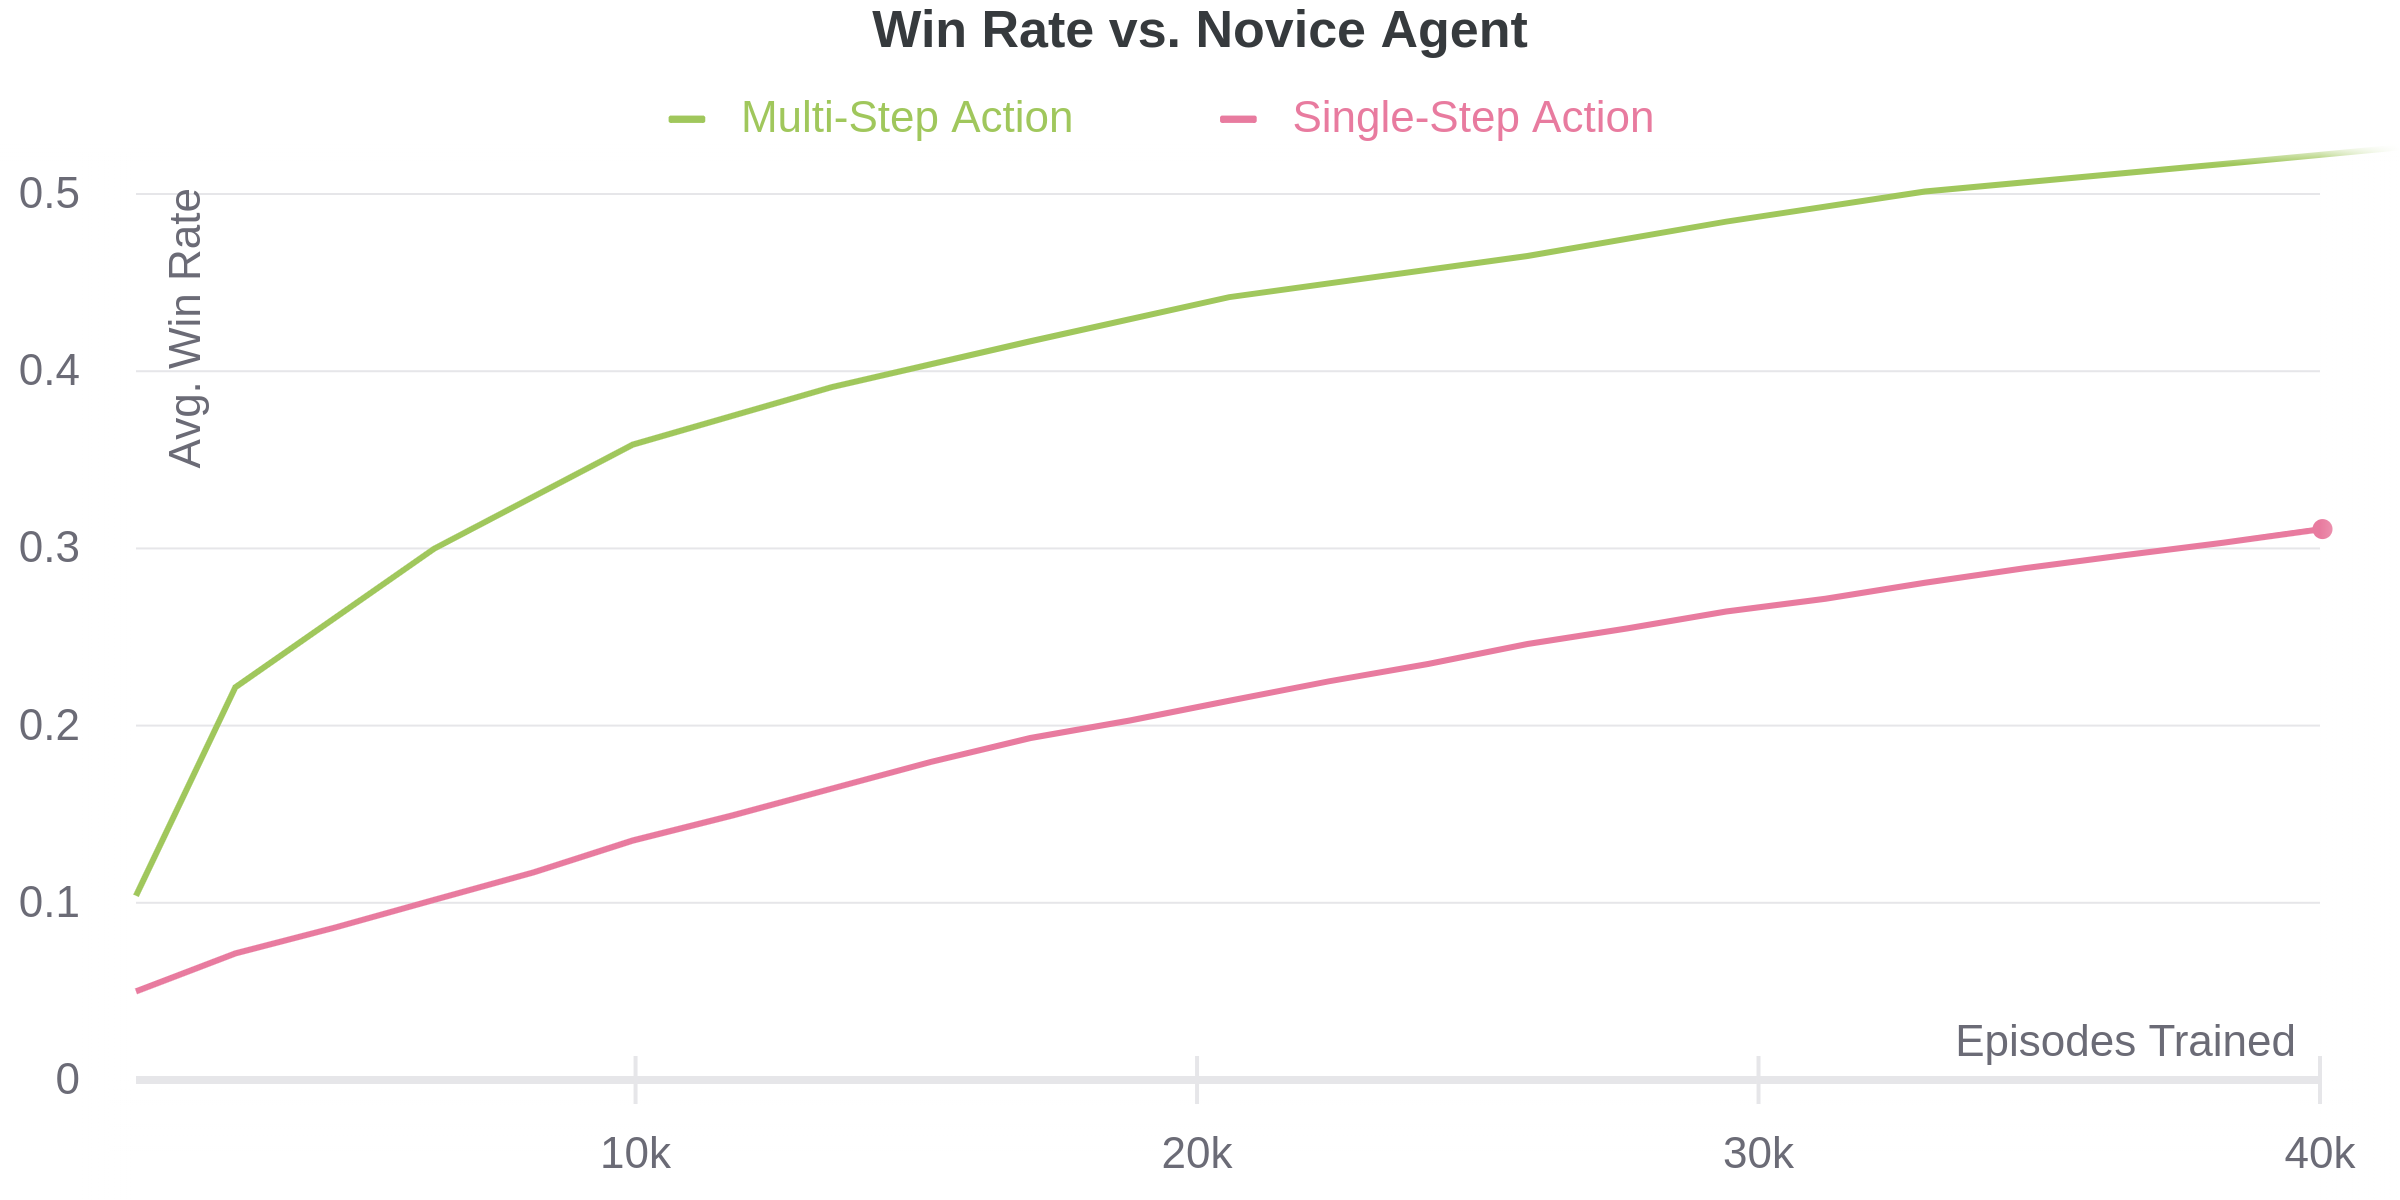
\includegraphics[width=\textwidth,keepaspectratio]{images/method/multi_vs_single_actions.png}
    \caption{Win rate vs Episodes Trained. This uses the novice rule agent to evaluate its performance for 500 episodes. This compares the two different action designs, single-step (where both discard and draw actions are taken together) and the opposite, multi-step.}
    \label{fig:multi_vs_single_actions}
\end{figure}


\subsubsection{Reward Function}
% \note{from james: Assumption about the readers knowledge. They may not know what a reward function is}

Reward shaping is another important part of the gym interface. The reward function is what determines the reward given to an agent when they do an action. It is possible to use dense rewards, which give a reward signal to the agent at every step, or more sparse rewards where an agent takes many steps before receiving a reward. The reward signal is extremely important \cite{li_deep_2018}, as it's what the agent uses to learn, it's what the agent is trying to maximise. 

Yaniv is a relatively simple game where the reward comes at the end. Either the agent wins, loses, or the game runs out of cards and a draw is called. The simplest reward scheme would assign a reward of +1 for a win, -1 for a loss, and zero for a draw \cite{warchalski_deep_2020}.

At the end of a Yaniv hand, the losers score points based on what is left in their hand. This number contributes to an overall game, where the aim is to score as few points as possible. To integrate this into the learning scheme a different reward function is proposed. 

\begin{equation}
r = \begin{cases}
    max(losingScores) / scoreCutoff & \text{if win} \\
                                   0 & \text{if draw} \\
    losingScore / scoreCutoff   & \text{if loss}
    \end{cases}
\label{eqn:reward_1}
\end{equation}

The reward described in \eqref{eqn:reward_1} is proportional to the scores at the end of the hand. The losers of the game score their hand divided by the cut-off variable and the winner scores the absolute value of the minimum reward. The score cut-off is set at 30. The aim of an agent is to maximise the score of the opponent, whilst minimising its own score. Losing by -2 has far less impact on the overall game than losing by -20. This reward scheme tries to incentivize agents to cause their opponent to lose by as large a score as possible, whilst minimizing its own losses, either by winning or scoring low.

\begin{figure}
    \centering
    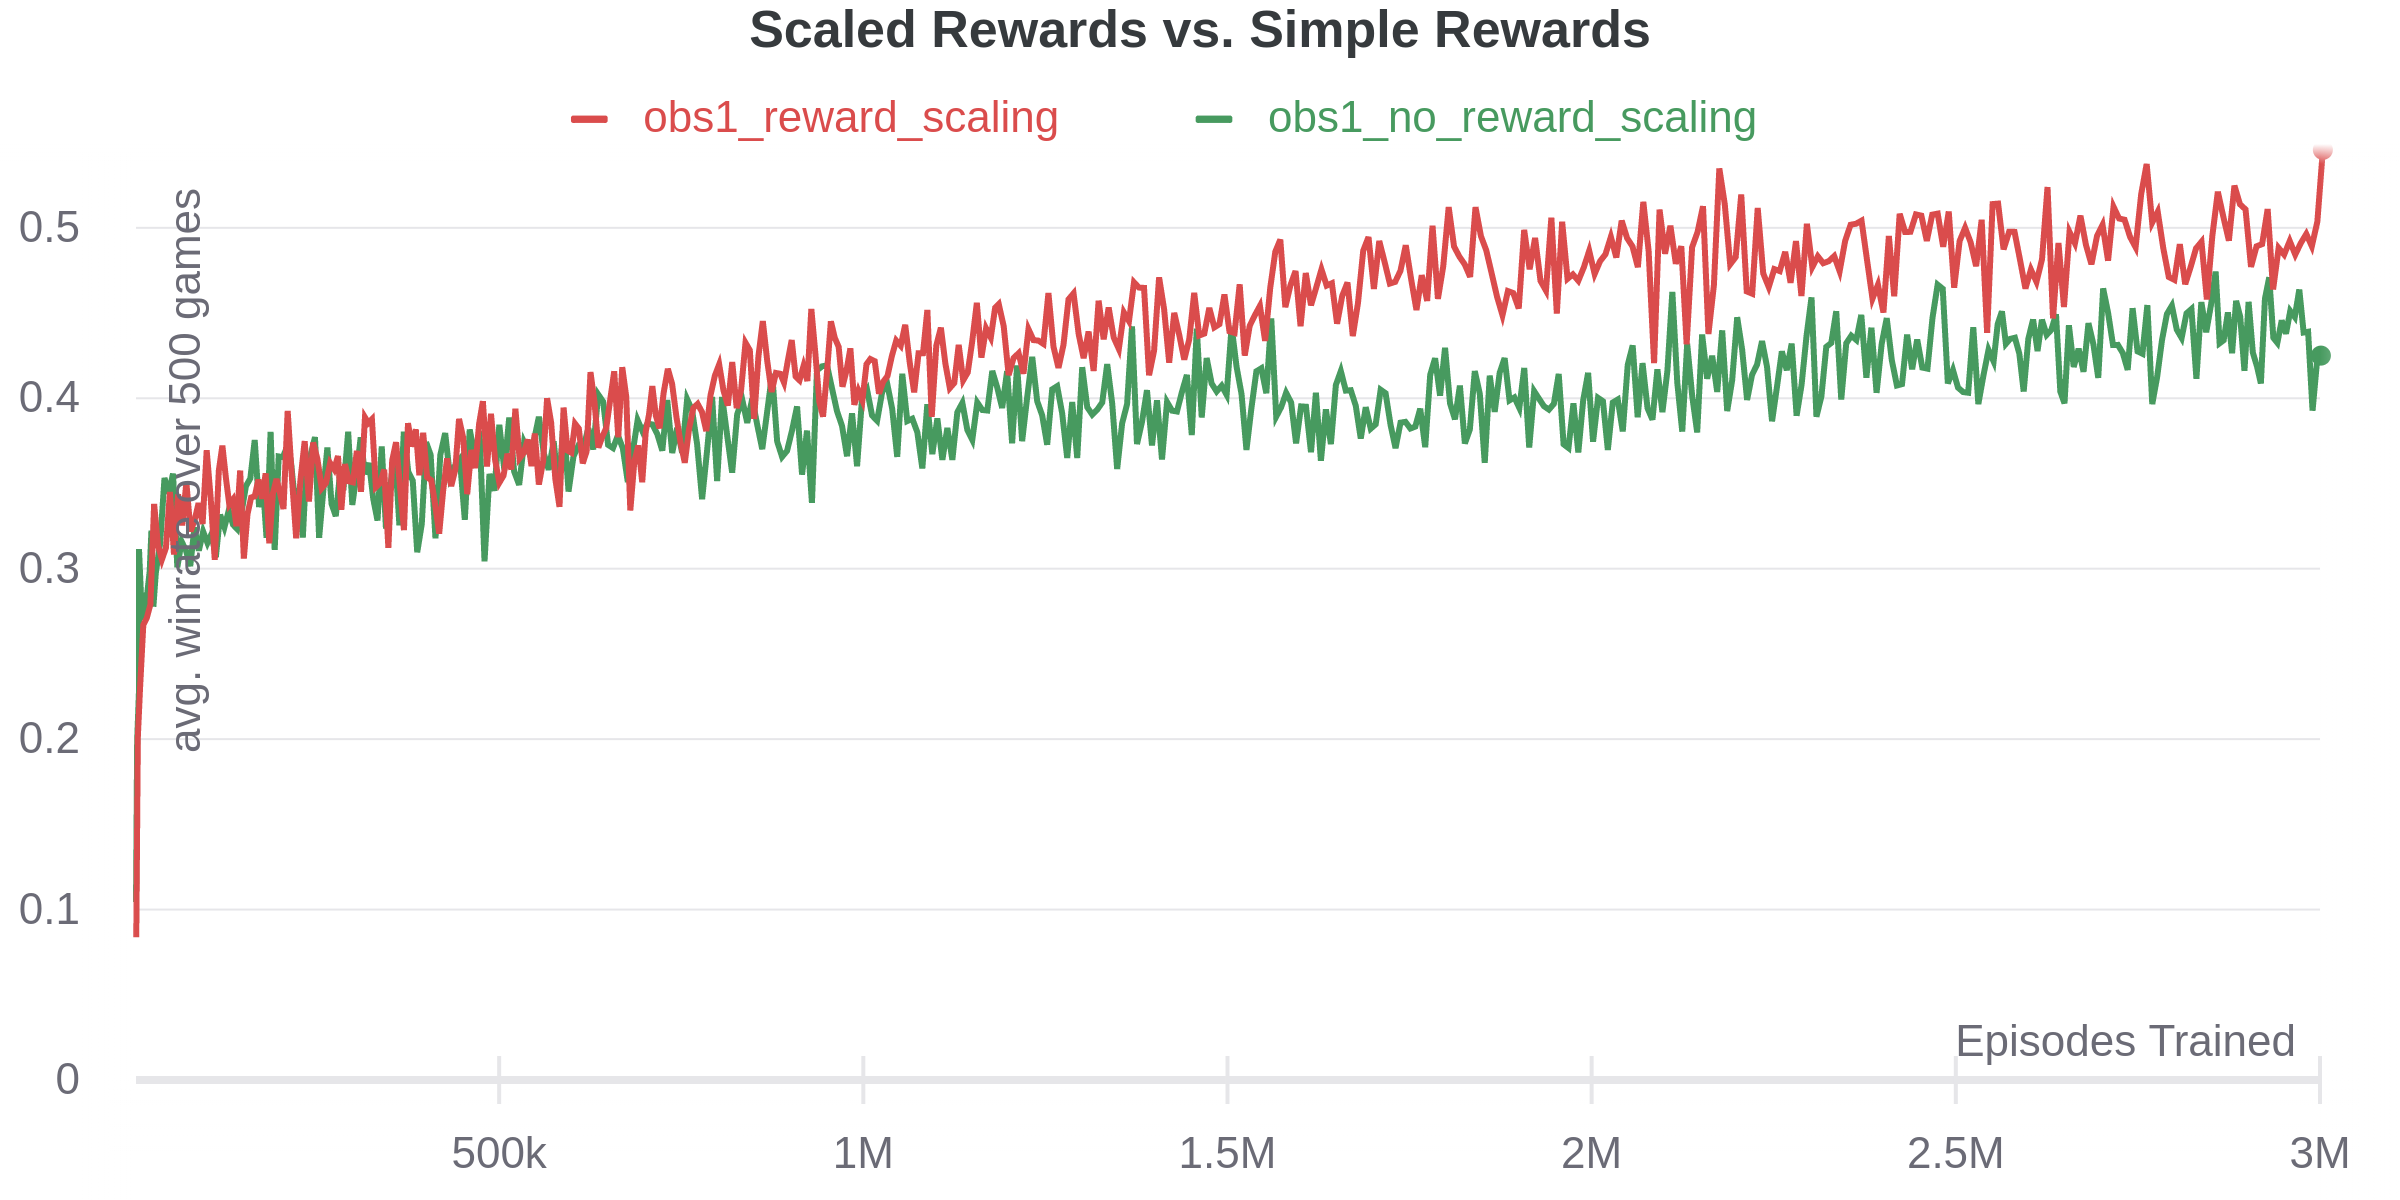
\includegraphics[width=\textwidth,keepaspectratio]{images/method/obs1_reward_scaling_comp.png}
    \caption{Win rate vs Training Iteration. The win rate is calculated over 500 games against an evaluation agent policy trained for ~10M episodes. Both plots use A3C. Represents ~20 hours of training time.}
    \label{fig:reward_scheme_comp}
\end{figure}

\cref{fig:reward_scheme_comp} shows the impact good reward shaping has on the training outcome. The green plot uses the simple reward scheme and the red plot uses \eqref{eqn:reward_1}. The reward scaling idea means that an agent isn't penalised for getting close to winning, which happens with the simple reward scheme. Equation \eqref{eqn:reward_1} more accurately describes the goal of the game - to reduce the overall score of your hand. 

\subsection{Training RL Agents}
To streamline the development process this project uses RLlib and Ray as the RL and distributed computing framework \cite{liang_rllib_2018}. RLlib has implemented and benchmarked many popular RL algorithms.

% \note{from James: Need to be more detailed here about why the two algorithms were chosen. Should include a comparison graph}

For this project I decided to use two actor-critic methods PPO \cite{schulman_proximal_2017} and A3C \cite{mnih_asynchronous_2016}. They're both online policy gradient algorithms. 

\begin{figure}
    \centering
    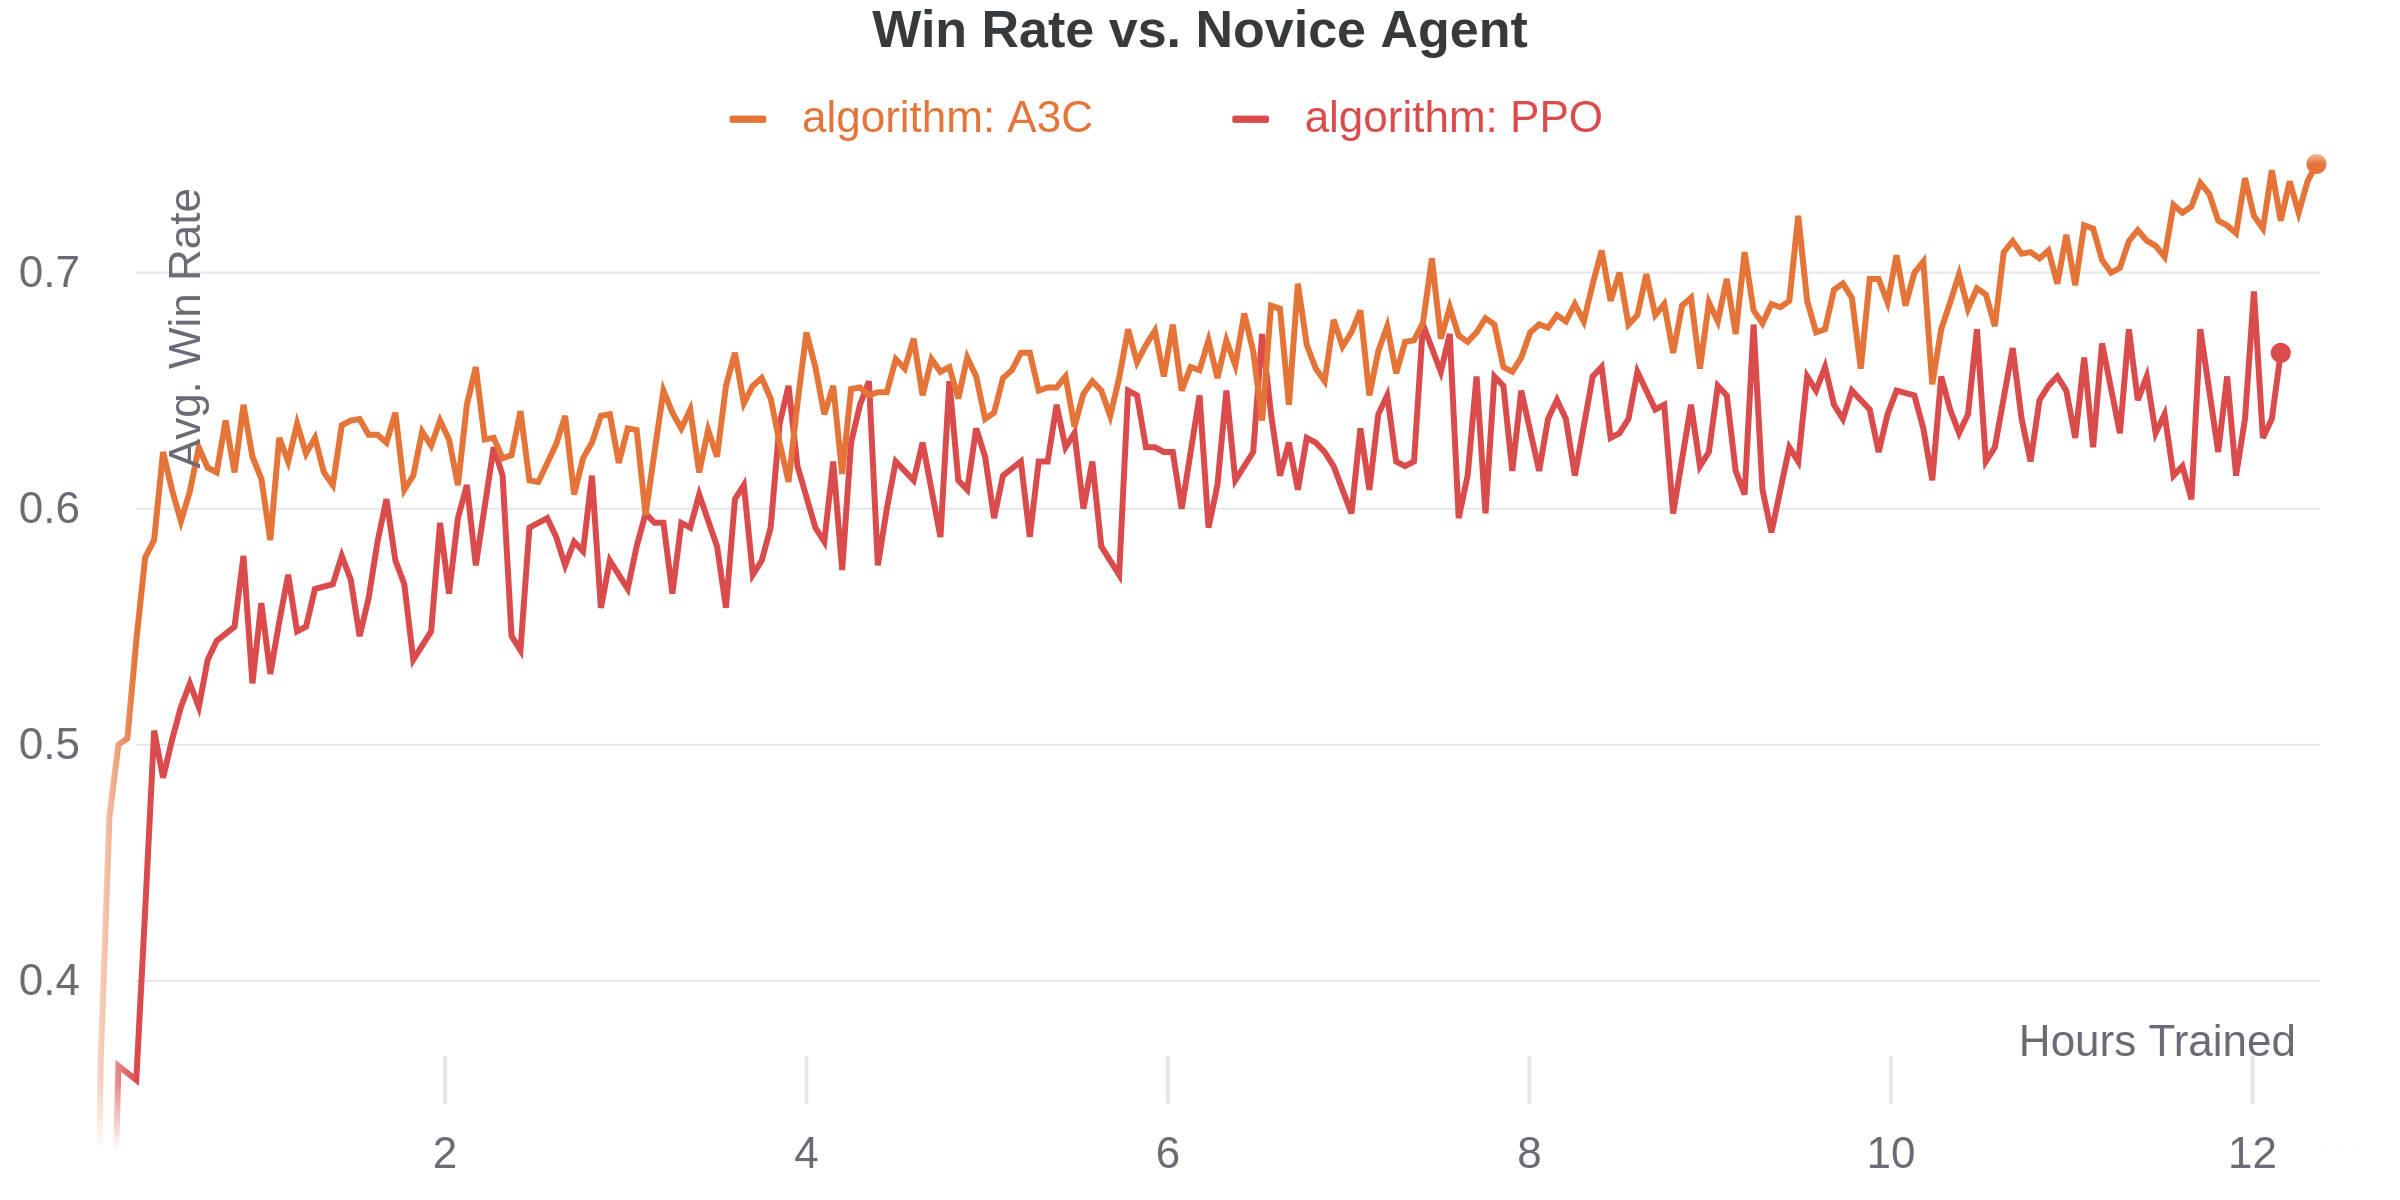
\includegraphics[width=\textwidth]{images/method/ppo_vs_a3c.png}
    \caption{Comparison of the A3C and PPO algorithm trained in 2 player. The win rate is calculated over 500 games against an evaluation agent policy trained over 12 hours.}
    \label{fig:ppo-vs-a3c}
\end{figure}


\subsubsection{Self-play} \label{method:selfplay}
% \note{from James: again too much background knowledge. Cross-ref back to the literature review and explain why to use self-play vs why not}

I implemented $\delta$-Uniform Self-Play with a small menagerie size of 4 due to low compute resources \cite{hernandez_comparison_2020}. The scheme trains policy 0 and uses it as player 0 when collecting samples. The opponents are sampled uniformly from the menagerie, which is populated with historical versions of policy 0 \cite{bansal_emergent_2018}. The gating function is as follows: if, after a training iteration, the trained policy has an average win rate of >0.55 then insert it into the menagerie. 

As described in \cref{litrev:self-play}, this means that during training the agent will play against historical versions of itself. This is so that as the agent grows in skill, so does the challenge. The reason to sample historical policies is to ensure that the agent does not \textit{forgot} older strategies. 

\subsubsection{Training}
Agents were trained over a series of environment configurations and hyperparameters. Overall the A3C algorithm performed best with the limited hyperparameter search I was able to conduct. It is simple and robust enough to provide suitable defaults out of the box, only needing to tune batch size parameters to achieve desirable results. PPO also offered a good option, but it is more sensitive to hyperparameters and with my limited compute resources tuning was difficult. A3C is slightly better suited as it scales better with CPUs versus PPO. A comparison of the two is shown in \cref{fig:ppo-vs-a3c}.

A3C is able to converge to a good level of play quicker than PPO, and then reaches a higher plateau. For this reason the rest of the experiments are done using A3C, as it trained quicker on the resources I had available with minimal hyperparameter tuning. 

In order to run experiments I had to chose one model which performed best and had historical policies saved. The configuration is listed in \cref{apx:training-config}. The model's policy is saved every 10 training steps (approximately 3,000 episodes.) \cref{fig:model_vs_rules} shows the results of training over 10k steps. 

\begin{figure}
    \centering
    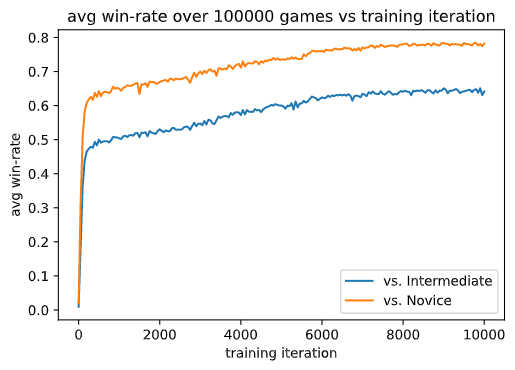
\includegraphics[width=\textwidth,keepaspectratio]{images/method/rules_vs_models.png}
    \caption{Performance of the model over training iteration. Evaluated at every 100th iteration against the novice and intermediate heuristic agent for 100,000 games. Trained with the configuration listed in \cref{apx:training-config}.}
    \label{fig:model_vs_rules}
\end{figure}

% \begin{figure}
%     \centering
%     \begin{subfigure}[t]{0.49\textwidth}
%         \centering
%         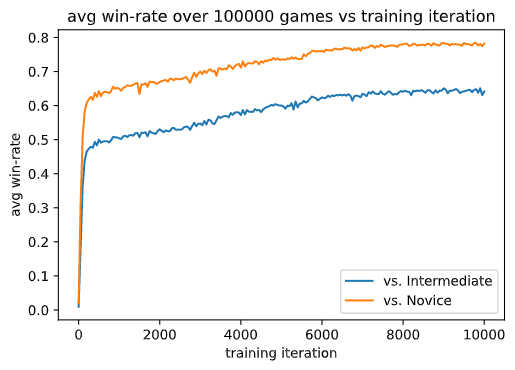
\includegraphics[width=\textwidth,keepaspectratio]{images/method/rules_vs_models.png}
%         \caption{Performance of the model over training iteration. Evaluated at every 100th iteration against the novice and intermediate heuristic agent for 100,000 games.}
%         \label{fig:model_vs_rules}
%     \end{subfigure}
%     \begin{subtable}[t]{0.49\textwidth}
%         \centering
%         \begin{tabular}[b]{@{}ll@{}}
%             \toprule
%             opponent     & win rate \\ \midrule
%             self         & 0.5      \\
%             random       & 0.5      \\
%             novice       & 0.5      \\
%             intermediate & 0.5      \\ \bottomrule
%         \end{tabular}
%         \caption{Mean win rate of the final model (trained for 10000 iterations) versus the rule agents. Each match up consists of 100000 simulated games.}
%         \label{tab:model-vs-rules}
%     \end{subtable}
% \end{figure}


\subfile{experiment_design}
\end{document}